\documentclass[1p]{elsarticle_modified}
%\bibliographystyle{elsarticle-num}

%\usepackage[colorlinks]{hyperref}
%\usepackage{abbrmath_seonhwa} %\Abb, \Ascr, \Acal ,\Abf, \Afrak
\usepackage{amsfonts}
\usepackage{amssymb}
\usepackage{amsmath}
\usepackage{amsthm}
\usepackage{scalefnt}
\usepackage{amsbsy}
\usepackage{kotex}
\usepackage{caption}
\usepackage{subfig}
\usepackage{color}
\usepackage{graphicx}
\usepackage{xcolor} %% white, black, red, green, blue, cyan, magenta, yellow
\usepackage{float}
\usepackage{setspace}
\usepackage{hyperref}

\usepackage{tikz}
\usetikzlibrary{arrows}

\usepackage{multirow}
\usepackage{array} % fixed length table
\usepackage{hhline}

%%%%%%%%%%%%%%%%%%%%%
\makeatletter
\renewcommand*\env@matrix[1][\arraystretch]{%
	\edef\arraystretch{#1}%
	\hskip -\arraycolsep
	\let\@ifnextchar\new@ifnextchar
	\array{*\c@MaxMatrixCols c}}
\makeatother %https://tex.stackexchange.com/questions/14071/how-can-i-increase-the-line-spacing-in-a-matrix
%%%%%%%%%%%%%%%

\usepackage[normalem]{ulem}

\newcommand{\msout}[1]{\ifmmode\text{\sout{\ensuremath{#1}}}\else\sout{#1}\fi}
%SOURCE: \msout is \stkout macro in https://tex.stackexchange.com/questions/20609/strikeout-in-math-mode

\newcommand{\cancel}[1]{
	\ifmmode
	{\color{red}\msout{#1}}
	\else
	{\color{red}\sout{#1}}
	\fi
}

\newcommand{\add}[1]{
	{\color{blue}\uwave{#1}}
}

\newcommand{\replace}[2]{
	\ifmmode
	{\color{red}\msout{#1}}{\color{blue}\uwave{#2}}
	\else
	{\color{red}\sout{#1}}{\color{blue}\uwave{#2}}
	\fi
}

\newcommand{\Sol}{\mathcal{S}} %segment
\newcommand{\D}{D} %diagram
\newcommand{\A}{\mathcal{A}} %arc


%%%%%%%%%%%%%%%%%%%%%%%%%%%%%5 test

\def\sl{\operatorname{\textup{SL}}(2,\Cbb)}
\def\psl{\operatorname{\textup{PSL}}(2,\Cbb)}
\def\quan{\mkern 1mu \triangleright \mkern 1mu}

\theoremstyle{definition}
\newtheorem{thm}{Theorem}[section]
\newtheorem{prop}[thm]{Proposition}
\newtheorem{lem}[thm]{Lemma}
\newtheorem{ques}[thm]{Question}
\newtheorem{cor}[thm]{Corollary}
\newtheorem{defn}[thm]{Definition}
\newtheorem{exam}[thm]{Example}
\newtheorem{rmk}[thm]{Remark}
\newtheorem{alg}[thm]{Algorithm}

\newcommand{\I}{\sqrt{-1}}
\begin{document}

%\begin{frontmatter}
%
%\title{Boundary parabolic representations of knots up to 8 crossings}
%
%%% Group authors per affiliation:
%\author{Yunhi Cho} 
%\address{Department of Mathematics, University of Seoul, Seoul, Korea}
%\ead{yhcho@uos.ac.kr}
%
%
%\author{Seonhwa Kim} %\fnref{s_kim}}
%\address{Center for Geometry and Physics, Institute for Basic Science, Pohang, 37673, Korea}
%\ead{ryeona17@ibs.re.kr}
%
%\author{Hyuk Kim}
%\address{Department of Mathematical Sciences, Seoul National University, Seoul 08826, Korea}
%\ead{hyukkim@snu.ac.kr}
%
%\author{Seokbeom Yoon}
%\address{Department of Mathematical Sciences, Seoul National University, Seoul, 08826,  Korea}
%\ead{sbyoon15@snu.ac.kr}
%
%\begin{abstract}
%We find all boundary parabolic representation of knots up to 8 crossings.
%
%\end{abstract}
%\begin{keyword}
%    \MSC[2010] 57M25 
%\end{keyword}
%
%\end{frontmatter}

%\linenumbers
%\tableofcontents
%
\newcommand\colored[1]{\textcolor{white}{\rule[-0.35ex]{0.8em}{1.4ex}}\kern-0.8em\color{red} #1}%
%\newcommand\colored[1]{\textcolor{white}{ #1}\kern-2.17ex	\textcolor{white}{ #1}\kern-1.81ex	\textcolor{white}{ #1}\kern-2.15ex\color{red}#1	}

{\Large $\underline{12n_{0346}~(K12n_{0346})}$}

\setlength{\tabcolsep}{10pt}
\renewcommand{\arraystretch}{1.6}
\vspace{1cm}\begin{tabular}{m{100pt}>{\centering\arraybackslash}m{274pt}}
\multirow{5}{120pt}{
	\centering
	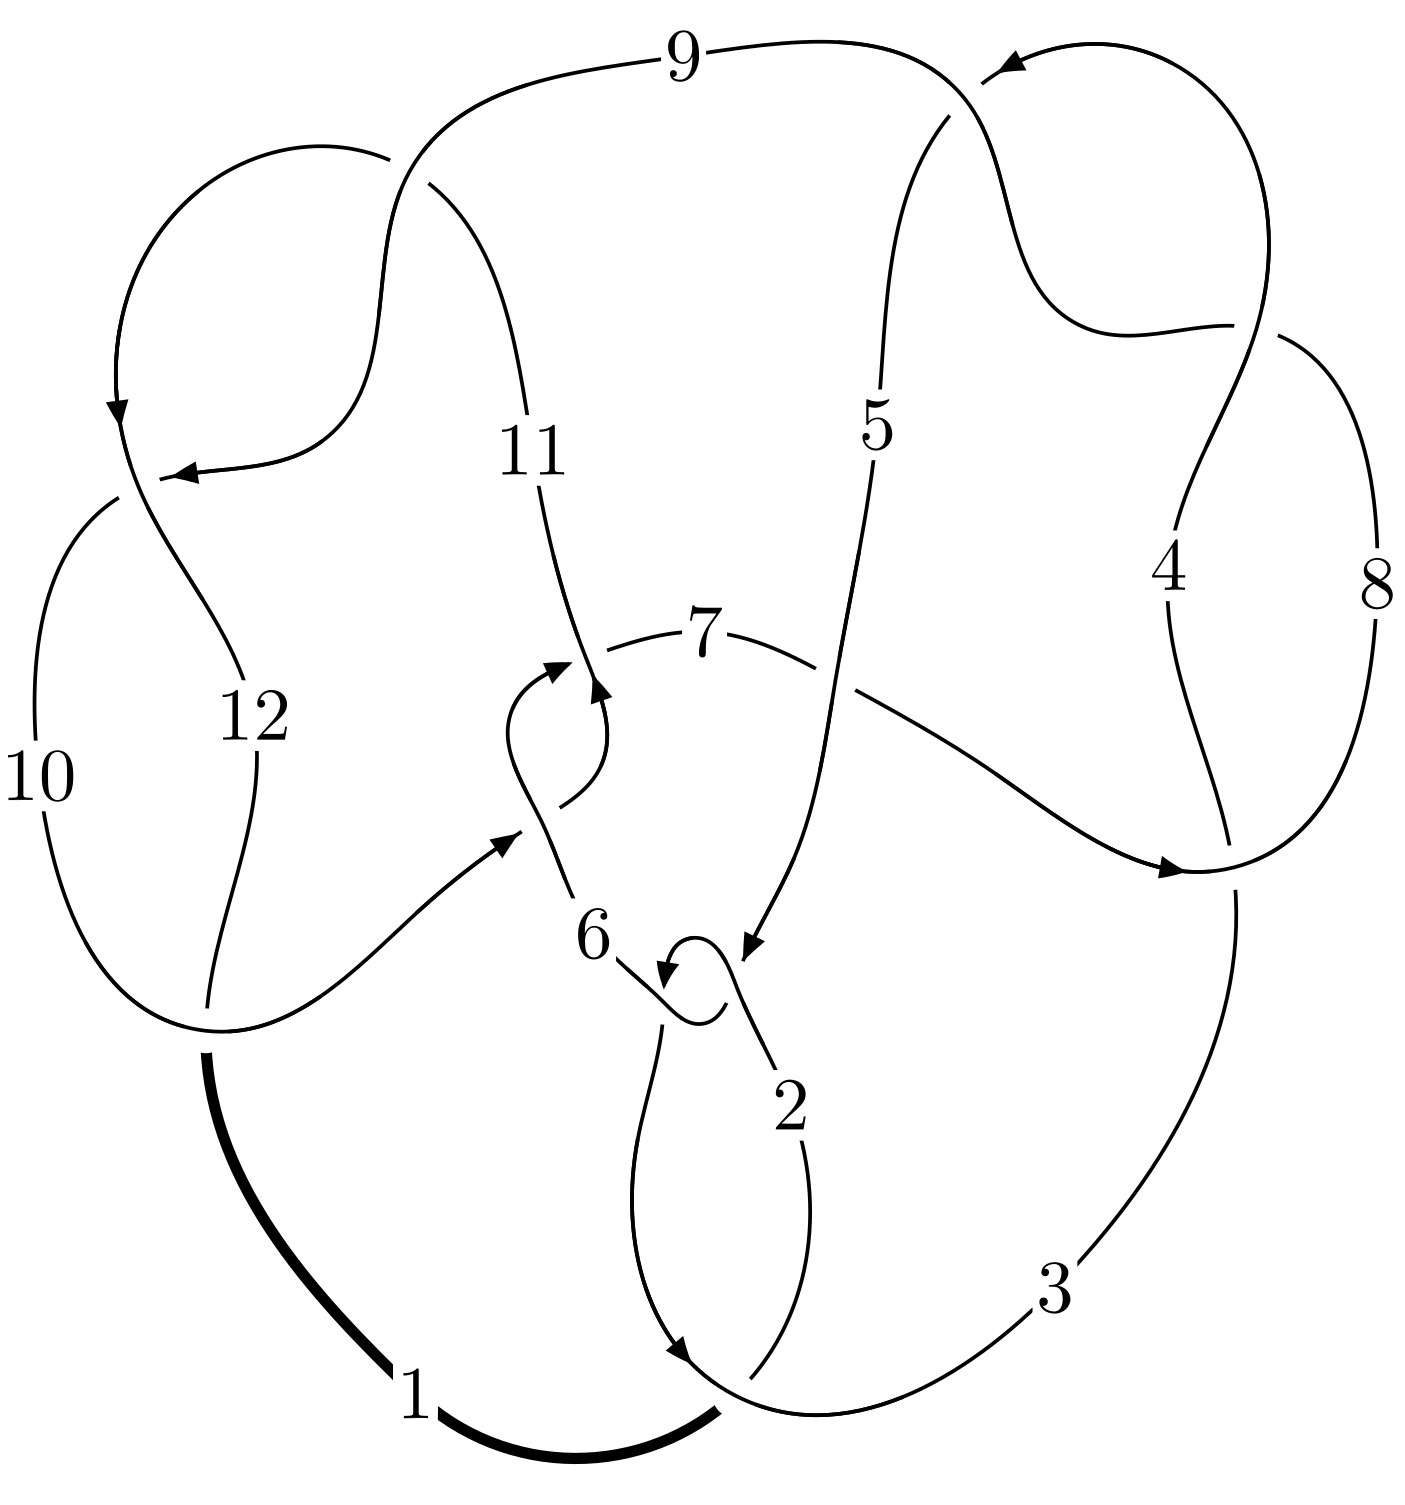
\includegraphics[width=112pt]{../../../GIT/diagram.site/Diagrams/png/2435_12n_0346.png}\\
\ \ \ A knot diagram\footnotemark}&
\allowdisplaybreaks
\textbf{Linearized knot diagam} \\
\cline{2-2}
 &
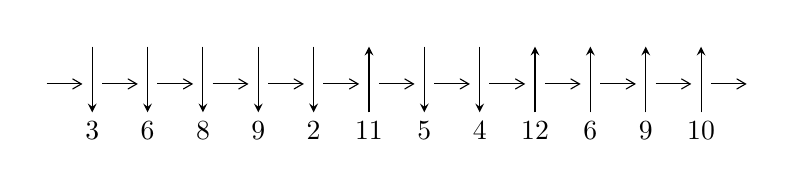
\begin{tikzpicture}[x=20pt, y=17pt]
	% nodes
	\node (C0) at (0, 0) {};
	\node (C1) at (1, 0) {};
	\node (C1U) at (1, +1) {};
	\node (C1D) at (1, -1) {3};

	\node (C2) at (2, 0) {};
	\node (C2U) at (2, +1) {};
	\node (C2D) at (2, -1) {6};

	\node (C3) at (3, 0) {};
	\node (C3U) at (3, +1) {};
	\node (C3D) at (3, -1) {8};

	\node (C4) at (4, 0) {};
	\node (C4U) at (4, +1) {};
	\node (C4D) at (4, -1) {9};

	\node (C5) at (5, 0) {};
	\node (C5U) at (5, +1) {};
	\node (C5D) at (5, -1) {2};

	\node (C6) at (6, 0) {};
	\node (C6U) at (6, +1) {};
	\node (C6D) at (6, -1) {11};

	\node (C7) at (7, 0) {};
	\node (C7U) at (7, +1) {};
	\node (C7D) at (7, -1) {5};

	\node (C8) at (8, 0) {};
	\node (C8U) at (8, +1) {};
	\node (C8D) at (8, -1) {4};

	\node (C9) at (9, 0) {};
	\node (C9U) at (9, +1) {};
	\node (C9D) at (9, -1) {12};

	\node (C10) at (10, 0) {};
	\node (C10U) at (10, +1) {};
	\node (C10D) at (10, -1) {6};

	\node (C11) at (11, 0) {};
	\node (C11U) at (11, +1) {};
	\node (C11D) at (11, -1) {9};

	\node (C12) at (12, 0) {};
	\node (C12U) at (12, +1) {};
	\node (C12D) at (12, -1) {10};
	\node (C13) at (13, 0) {};

	% arrows
	\draw[->,>={angle 60}]
	(C0) edge (C1) (C1) edge (C2) (C2) edge (C3) (C3) edge (C4) (C4) edge (C5) (C5) edge (C6) (C6) edge (C7) (C7) edge (C8) (C8) edge (C9) (C9) edge (C10) (C10) edge (C11) (C11) edge (C12) (C12) edge (C13) ;	\draw[->,>=stealth]
	(C1U) edge (C1D) (C2U) edge (C2D) (C3U) edge (C3D) (C4U) edge (C4D) (C5U) edge (C5D) (C6D) edge (C6U) (C7U) edge (C7D) (C8U) edge (C8D) (C9D) edge (C9U) (C10D) edge (C10U) (C11D) edge (C11U) (C12D) edge (C12U) ;
	\end{tikzpicture} \\
\hhline{~~} \\& 
\textbf{Solving Sequence} \\ \cline{2-2} 
 &
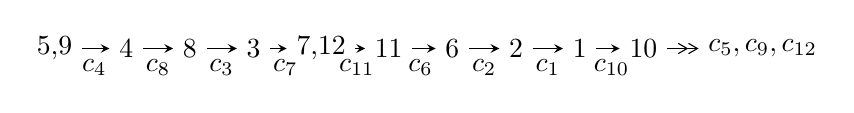
\begin{tikzpicture}[x=23pt, y=7pt]
	% node
	\node (A0) at (-1/8, 0) {5,9};
	\node (A1) at (1, 0) {4};
	\node (A2) at (2, 0) {8};
	\node (A3) at (3, 0) {3};
	\node (A4) at (65/16, 0) {7,12};
	\node (A5) at (41/8, 0) {11};
	\node (A6) at (49/8, 0) {6};
	\node (A7) at (57/8, 0) {2};
	\node (A8) at (65/8, 0) {1};
	\node (A9) at (73/8, 0) {10};
	\node (C1) at (1/2, -1) {$c_{4}$};
	\node (C2) at (3/2, -1) {$c_{8}$};
	\node (C3) at (5/2, -1) {$c_{3}$};
	\node (C4) at (7/2, -1) {$c_{7}$};
	\node (C5) at (37/8, -1) {$c_{11}$};
	\node (C6) at (45/8, -1) {$c_{6}$};
	\node (C7) at (53/8, -1) {$c_{2}$};
	\node (C8) at (61/8, -1) {$c_{1}$};
	\node (C9) at (69/8, -1) {$c_{10}$};
	\node (A10) at (11, 0) {$c_{5},c_{9},c_{12}$};

	% edge
	\draw[->,>=stealth]	
	(A0) edge (A1) (A1) edge (A2) (A2) edge (A3) (A3) edge (A4) (A4) edge (A5) (A5) edge (A6) (A6) edge (A7) (A7) edge (A8) (A8) edge (A9) ;
	\draw[->>,>={angle 60}]	
	(A9) edge (A10);
\end{tikzpicture} \\ 

\end{tabular} \\

\footnotetext{
The image of knot diagram is generated by the software ``\textbf{Draw programme}" developed by Andrew Bartholomew(\url{http://www.layer8.co.uk/maths/draw/index.htm\#Running-draw}), where we modified some parts for our purpose(\url{https://github.com/CATsTAILs/LinksPainter}).
}\phantom \\ \newline 
\centering \textbf{Ideals for irreducible components\footnotemark of $X_{\text{par}}$} 
 
\begin{align*}
I^u_{1}&=\langle 
-8563315867395 u^{19}+12169590007513 u^{18}+\cdots+13082431761068 b+64802000815324,\\
\phantom{I^u_{1}}&\phantom{= \langle  }52899877847623 u^{19}-79722292100065 u^{18}+\cdots+13082431761068 a-413103210378158,\\
\phantom{I^u_{1}}&\phantom{= \langle  }u^{20}-2 u^{19}+\cdots-12 u+4\rangle \\
I^u_{2}&=\langle 
u^7- u^6-2 u^5+3 u^4-2 u^2+b+4 u-2,\;- u^7- u^6+3 u^5+2 u^4-3 u^3+a-2,\\
\phantom{I^u_{2}}&\phantom{= \langle  }u^8+u^7-3 u^6-2 u^5+3 u^4+2 u-1\rangle \\
I^u_{3}&=\langle 
- a u+b- u-1,\;2 a^2+a u-1,\;u^2-2\rangle \\
\\
I^v_{1}&=\langle 
a,\;b- v+2,\;v^2-3 v+1\rangle \\
\end{align*}
\raggedright * 4 irreducible components of $\dim_{\mathbb{C}}=0$, with total 34 representations.\\
\footnotetext{All coefficients of polynomials are rational numbers. But the coefficients are sometimes approximated in decimal forms when there is not enough margin.}
\newpage
\renewcommand{\arraystretch}{1}
\centering \section*{I. $I^u_{1}= \langle -8.56\times10^{12} u^{19}+1.22\times10^{13} u^{18}+\cdots+1.31\times10^{13} b+6.48\times10^{13},\;5.29\times10^{13} u^{19}-7.97\times10^{13} u^{18}+\cdots+1.31\times10^{13} a-4.13\times10^{14},\;u^{20}-2 u^{19}+\cdots-12 u+4 \rangle$}
\flushleft \textbf{(i) Arc colorings}\\
\begin{tabular}{m{7pt} m{180pt} m{7pt} m{180pt} }
\flushright $a_{5}=$&$\begin{pmatrix}1\\0\end{pmatrix}$ \\
\flushright $a_{9}=$&$\begin{pmatrix}0\\u\end{pmatrix}$ \\
\flushright $a_{4}=$&$\begin{pmatrix}1\\- u^2\end{pmatrix}$ \\
\flushright $a_{8}=$&$\begin{pmatrix}u\\- u^3+u\end{pmatrix}$ \\
\flushright $a_{3}=$&$\begin{pmatrix}- u^2+1\\u^4-2 u^2\end{pmatrix}$ \\
\flushright $a_{7}=$&$\begin{pmatrix}- u^3+2 u\\- u^3+u\end{pmatrix}$ \\
\flushright $a_{12}=$&$\begin{pmatrix}-4.04358 u^{19}+6.09384 u^{18}+\cdots-25.5560 u+31.5769\\0.654566 u^{19}-0.930224 u^{18}+\cdots+6.84847 u-4.95336\end{pmatrix}$ \\
\flushright $a_{11}=$&$\begin{pmatrix}-4.04358 u^{19}+6.09384 u^{18}+\cdots-25.5560 u+31.5769\\-0.367222 u^{19}+0.611916 u^{18}+\cdots-0.897037 u+3.01992\end{pmatrix}$ \\
\flushright $a_{6}=$&$\begin{pmatrix}-6.21544 u^{19}+9.28273 u^{18}+\cdots-48.2193 u+51.0252\\0.348398 u^{19}-0.661202 u^{18}+\cdots+3.63448 u-3.80249\end{pmatrix}$ \\
\flushright $a_{2}=$&$\begin{pmatrix}-4.90774 u^{19}+7.58167 u^{18}+\cdots-38.9378 u+42.2351\\2.23801 u^{19}-3.26288 u^{18}+\cdots+16.4563 u-17.7254\end{pmatrix}$ \\
\flushright $a_{1}=$&$\begin{pmatrix}-5.35239 u^{19}+8.30016 u^{18}+\cdots-43.5388 u+45.8952\\2.16712 u^{19}-3.30945 u^{18}+\cdots+15.7609 u-18.5509\end{pmatrix}$ \\
\flushright $a_{10}=$&$\begin{pmatrix}5.60383 u^{19}-8.48450 u^{18}+\cdots+48.3882 u-47.1067\\-2.25347 u^{19}+3.54770 u^{18}+\cdots-15.9192 u+19.1670\end{pmatrix}$\\&\end{tabular}
\flushleft \textbf{(ii) Obstruction class $= -1$}\\~\\
\flushleft \textbf{(iii) Cusp Shapes $= \frac{8651471282093}{3270607940267} u^{19}-\frac{12603254258761}{3270607940267} u^{18}+\cdots-\frac{78299168927818}{3270607940267} u-\frac{83998088848016}{3270607940267}$}\\~\\
\newpage\renewcommand{\arraystretch}{1}
\flushleft \textbf{(iv) u-Polynomials at the component}\newline \\
\begin{tabular}{m{50pt}|m{274pt}}
Crossings & \hspace{64pt}u-Polynomials at each crossing \\
\hline $$\begin{aligned}c_{1}\end{aligned}$$&$\begin{aligned}
&u^{20}+24 u^{18}+\cdots+3807 u+81
\end{aligned}$\\
\hline $$\begin{aligned}c_{2},c_{5}\end{aligned}$$&$\begin{aligned}
&u^{20}+4 u^{19}+\cdots-93 u-9
\end{aligned}$\\
\hline $$\begin{aligned}c_{3},c_{4},c_{8}\end{aligned}$$&$\begin{aligned}
&u^{20}+2 u^{19}+\cdots+12 u+4
\end{aligned}$\\
\hline $$\begin{aligned}c_{6},c_{10}\end{aligned}$$&$\begin{aligned}
&u^{20}+2 u^{19}+\cdots+3200 u+256
\end{aligned}$\\
\hline $$\begin{aligned}c_{7}\end{aligned}$$&$\begin{aligned}
&u^{20}-6 u^{19}+\cdots-6212 u-964
\end{aligned}$\\
\hline $$\begin{aligned}c_{9},c_{11},c_{12}\end{aligned}$$&$\begin{aligned}
&u^{20}+12 u^{19}+\cdots-58 u+1
\end{aligned}$\\
\hline
\end{tabular}\\~\\
\newpage\renewcommand{\arraystretch}{1}
\flushleft \textbf{(v) Riley Polynomials at the component}\newline \\
\begin{tabular}{m{50pt}|m{274pt}}
Crossings & \hspace{64pt}Riley Polynomials at each crossing \\
\hline $$\begin{aligned}c_{1}\end{aligned}$$&$\begin{aligned}
&y^{20}+48 y^{19}+\cdots-10684791 y+6561
\end{aligned}$\\
\hline $$\begin{aligned}c_{2},c_{5}\end{aligned}$$&$\begin{aligned}
&y^{20}+24 y^{18}+\cdots-3807 y+81
\end{aligned}$\\
\hline $$\begin{aligned}c_{3},c_{4},c_{8}\end{aligned}$$&$\begin{aligned}
&y^{20}-14 y^{19}+\cdots-432 y+16
\end{aligned}$\\
\hline $$\begin{aligned}c_{6},c_{10}\end{aligned}$$&$\begin{aligned}
&y^{20}-60 y^{19}+\cdots-5160960 y+65536
\end{aligned}$\\
\hline $$\begin{aligned}c_{7}\end{aligned}$$&$\begin{aligned}
&y^{20}+58 y^{19}+\cdots-44905072 y+929296
\end{aligned}$\\
\hline $$\begin{aligned}c_{9},c_{11},c_{12}\end{aligned}$$&$\begin{aligned}
&y^{20}-44 y^{19}+\cdots-2922 y+1
\end{aligned}$\\
\hline
\end{tabular}\\~\\
\newpage\flushleft \textbf{(vi) Complex Volumes and Cusp Shapes}
$$\begin{array}{c|c|c}  
\text{Solutions to }I^u_{1}& \I (\text{vol} + \sqrt{-1}CS) & \text{Cusp shape}\\
 \hline 
\begin{aligned}
u &= -0.311540 + 0.820503 I \\
a &= -1.183960 + 0.104977 I \\
b &= -0.936205 - 0.261735 I\end{aligned}
 & \phantom{-}1.94026 - 0.82547 I & \phantom{-}0.912486 + 0.761117 I \\ \hline\begin{aligned}
u &= -0.311540 - 0.820503 I \\
a &= -1.183960 - 0.104977 I \\
b &= -0.936205 + 0.261735 I\end{aligned}
 & \phantom{-}1.94026 + 0.82547 I & \phantom{-}0.912486 - 0.761117 I \\ \hline\begin{aligned}
u &= \phantom{-}0.806269 + 0.099052 I \\
a &= -0.029427 - 0.611307 I \\
b &= \phantom{-}0.383913 - 0.245700 I\end{aligned}
 & -1.290640 + 0.060456 I & -5.65835 + 0.55419 I \\ \hline\begin{aligned}
u &= \phantom{-}0.806269 - 0.099052 I \\
a &= -0.029427 + 0.611307 I \\
b &= \phantom{-}0.383913 + 0.245700 I\end{aligned}
 & -1.290640 - 0.060456 I & -5.65835 - 0.55419 I \\ \hline\begin{aligned}
u &= \phantom{-}1.33638\phantom{ +0.000000I} \\
a &= -1.16154\phantom{ +0.000000I} \\
b &= \phantom{-}1.16836\phantom{ +0.000000I}\end{aligned}
 & \phantom{-}3.62783\phantom{ +0.000000I} & \phantom{-}3.71420\phantom{ +0.000000I} \\ \hline\begin{aligned}
u &= -1.301610 + 0.401831 I \\
a &= \phantom{-}0.508418 - 0.295516 I \\
b &= -0.439577 + 0.851076 I\end{aligned}
 & -1.51005 + 5.52302 I & -5.54282 - 3.24717 I \\ \hline\begin{aligned}
u &= -1.301610 - 0.401831 I \\
a &= \phantom{-}0.508418 + 0.295516 I \\
b &= -0.439577 - 0.851076 I\end{aligned}
 & -1.51005 - 5.52302 I & -5.54282 + 3.24717 I \\ \hline\begin{aligned}
u &= \phantom{-}1.037800 + 0.883330 I \\
a &= \phantom{-}0.77758 - 1.27910 I \\
b &= -2.72069 - 2.90147 I\end{aligned}
 & \phantom{-}4.14315 - 3.36874 I & \phantom{-}0.04800 + 2.58345 I \\ \hline\begin{aligned}
u &= \phantom{-}1.037800 - 0.883330 I \\
a &= \phantom{-}0.77758 + 1.27910 I \\
b &= -2.72069 + 2.90147 I\end{aligned}
 & \phantom{-}4.14315 + 3.36874 I & \phantom{-}0.04800 - 2.58345 I \\ \hline\begin{aligned}
u &= -1.38998\phantom{ +0.000000I} \\
a &= -0.0133698\phantom{ +0.000000I} \\
b &= -1.23390\phantom{ +0.000000I}\end{aligned}
 & -6.53389\phantom{ +0.000000I} & -14.0580\phantom{ +0.000000I}\\
 \hline 
 \end{array}$$\newpage$$\begin{array}{c|c|c}  
\text{Solutions to }I^u_{1}& \I (\text{vol} + \sqrt{-1}CS) & \text{Cusp shape}\\
 \hline 
\begin{aligned}
u &= -0.307583 + 1.370650 I \\
a &= \phantom{-}0.05460 + 1.81689 I \\
b &= -1.41200 + 5.33955 I\end{aligned}
 & -16.9450 + 5.1999 I & \phantom{-}0.48479 - 2.11695 I \\ \hline\begin{aligned}
u &= -0.307583 - 1.370650 I \\
a &= \phantom{-}0.05460 - 1.81689 I \\
b &= -1.41200 - 5.33955 I\end{aligned}
 & -16.9450 - 5.1999 I & \phantom{-}0.48479 + 2.11695 I \\ \hline\begin{aligned}
u &= \phantom{-}1.43456\phantom{ +0.000000I} \\
a &= \phantom{-}0.671677\phantom{ +0.000000I} \\
b &= \phantom{-}7.72000\phantom{ +0.000000I}\end{aligned}
 & -4.98064\phantom{ +0.000000I} & \phantom{-}60.9990\phantom{ +0.000000I} \\ \hline\begin{aligned}
u &= \phantom{-}0.486279\phantom{ +0.000000I} \\
a &= -3.47218\phantom{ +0.000000I} \\
b &= \phantom{-}1.37914\phantom{ +0.000000I}\end{aligned}
 & \phantom{-}6.88313\phantom{ +0.000000I} & -9.17840\phantom{ +0.000000I} \\ \hline\begin{aligned}
u &= \phantom{-}0.388073\phantom{ +0.000000I} \\
a &= \phantom{-}0.457271\phantom{ +0.000000I} \\
b &= \phantom{-}0.718784\phantom{ +0.000000I}\end{aligned}
 & -1.01688\phantom{ +0.000000I} & -12.8430\phantom{ +0.000000I} \\ \hline\begin{aligned}
u &= \phantom{-}1.58364 + 0.49918 I \\
a &= -1.064100 + 0.688577 I \\
b &= \phantom{-}3.34498 + 2.38478 I\end{aligned}
 & \phantom{-}16.4234 - 11.7755 I & -1.93237 + 4.54638 I \\ \hline\begin{aligned}
u &= \phantom{-}1.58364 - 0.49918 I \\
a &= -1.064100 - 0.688577 I \\
b &= \phantom{-}3.34498 - 2.38478 I\end{aligned}
 & \phantom{-}16.4234 + 11.7755 I & -1.93237 - 4.54638 I \\ \hline\begin{aligned}
u &= -0.283054\phantom{ +0.000000I} \\
a &= -3.06452\phantom{ +0.000000I} \\
b &= -0.370034\phantom{ +0.000000I}\end{aligned}
 & \phantom{-}1.22670\phantom{ +0.000000I} & \phantom{-}10.7000\phantom{ +0.000000I} \\ \hline\begin{aligned}
u &= -1.49310 + 0.84801 I \\
a &= \phantom{-}1.22823 + 0.86872 I \\
b &= -3.91160 + 3.62679 I\end{aligned}
 & \phantom{-}19.0199 + 2.7480 I & -0.478669 - 0.983748 I \\ \hline\begin{aligned}
u &= -1.49310 - 0.84801 I \\
a &= \phantom{-}1.22823 - 0.86872 I \\
b &= -3.91160 - 3.62679 I\end{aligned}
 & \phantom{-}19.0199 - 2.7480 I & -0.478669 + 0.983748 I\\
 \hline 
 \end{array}$$\newpage\newpage\renewcommand{\arraystretch}{1}
\centering \section*{II. $I^u_{2}= \langle u^7- u^6-2 u^5+3 u^4-2 u^2+b+4 u-2,\;- u^7- u^6+3 u^5+2 u^4-3 u^3+a-2,\;u^8+u^7-3 u^6-2 u^5+3 u^4+2 u-1 \rangle$}
\flushleft \textbf{(i) Arc colorings}\\
\begin{tabular}{m{7pt} m{180pt} m{7pt} m{180pt} }
\flushright $a_{5}=$&$\begin{pmatrix}1\\0\end{pmatrix}$ \\
\flushright $a_{9}=$&$\begin{pmatrix}0\\u\end{pmatrix}$ \\
\flushright $a_{4}=$&$\begin{pmatrix}1\\- u^2\end{pmatrix}$ \\
\flushright $a_{8}=$&$\begin{pmatrix}u\\- u^3+u\end{pmatrix}$ \\
\flushright $a_{3}=$&$\begin{pmatrix}- u^2+1\\u^4-2 u^2\end{pmatrix}$ \\
\flushright $a_{7}=$&$\begin{pmatrix}- u^3+2 u\\- u^3+u\end{pmatrix}$ \\
\flushright $a_{12}=$&$\begin{pmatrix}u^7+u^6-3 u^5-2 u^4+3 u^3+2\\- u^7+u^6+2 u^5-3 u^4+2 u^2-4 u+2\end{pmatrix}$ \\
\flushright $a_{11}=$&$\begin{pmatrix}u^7+u^6-3 u^5-2 u^4+3 u^3+2\\- u^7+u^6+2 u^5-3 u^4+2 u^2-3 u+2\end{pmatrix}$ \\
\flushright $a_{6}=$&$\begin{pmatrix}- u^3+2 u\\- u^3+u\end{pmatrix}$ \\
\flushright $a_{2}=$&$\begin{pmatrix}u^5-2 u^3+u\\- u^7+3 u^5-2 u^3- u\end{pmatrix}$ \\
\flushright $a_{1}=$&$\begin{pmatrix}0\\- u\end{pmatrix}$ \\
\flushright $a_{10}=$&$\begin{pmatrix}u^7+u^6-3 u^5-2 u^4+3 u^3+2\\- u^7+u^6+2 u^5-3 u^4+2 u^2-3 u+2\end{pmatrix}$\\&\end{tabular}
\flushleft \textbf{(ii) Obstruction class $= 1$}\\~\\
\flushleft \textbf{(iii) Cusp Shapes $= 4 u^7-9 u^6-10 u^5+27 u^4-2 u^3-18 u^2+20 u-17$}\\~\\
\newpage\renewcommand{\arraystretch}{1}
\flushleft \textbf{(iv) u-Polynomials at the component}\newline \\
\begin{tabular}{m{50pt}|m{274pt}}
Crossings & \hspace{64pt}u-Polynomials at each crossing \\
\hline $$\begin{aligned}c_{1}\end{aligned}$$&$\begin{aligned}
&u^8-3 u^7+7 u^6-10 u^5+11 u^4-10 u^3+6 u^2-4 u+1
\end{aligned}$\\
\hline $$\begin{aligned}c_{2}\end{aligned}$$&$\begin{aligned}
&u^8- u^7- u^6+2 u^5+u^4-2 u^3+2 u-1
\end{aligned}$\\
\hline $$\begin{aligned}c_{3},c_{4}\end{aligned}$$&$\begin{aligned}
&u^8+u^7-3 u^6-2 u^5+3 u^4+2 u-1
\end{aligned}$\\
\hline $$\begin{aligned}c_{5}\end{aligned}$$&$\begin{aligned}
&u^8+u^7- u^6-2 u^5+u^4+2 u^3-2 u-1
\end{aligned}$\\
\hline $$\begin{aligned}c_{6},c_{10}\end{aligned}$$&$\begin{aligned}
&u^8
\end{aligned}$\\
\hline $$\begin{aligned}c_{7}\end{aligned}$$&$\begin{aligned}
&u^8+3 u^7+7 u^6+10 u^5+11 u^4+10 u^3+6 u^2+4 u+1
\end{aligned}$\\
\hline $$\begin{aligned}c_{8}\end{aligned}$$&$\begin{aligned}
&u^8- u^7-3 u^6+2 u^5+3 u^4-2 u-1
\end{aligned}$\\
\hline $$\begin{aligned}c_{9}\end{aligned}$$&$\begin{aligned}
&(u+1)^8
\end{aligned}$\\
\hline $$\begin{aligned}c_{11},c_{12}\end{aligned}$$&$\begin{aligned}
&(u-1)^8
\end{aligned}$\\
\hline
\end{tabular}\\~\\
\newpage\renewcommand{\arraystretch}{1}
\flushleft \textbf{(v) Riley Polynomials at the component}\newline \\
\begin{tabular}{m{50pt}|m{274pt}}
Crossings & \hspace{64pt}Riley Polynomials at each crossing \\
\hline $$\begin{aligned}c_{1},c_{7}\end{aligned}$$&$\begin{aligned}
&y^8+5 y^7+11 y^6+6 y^5-17 y^4-34 y^3-22 y^2-4 y+1
\end{aligned}$\\
\hline $$\begin{aligned}c_{2},c_{5}\end{aligned}$$&$\begin{aligned}
&y^8-3 y^7+7 y^6-10 y^5+11 y^4-10 y^3+6 y^2-4 y+1
\end{aligned}$\\
\hline $$\begin{aligned}c_{3},c_{4},c_{8}\end{aligned}$$&$\begin{aligned}
&y^8-7 y^7+19 y^6-22 y^5+3 y^4+14 y^3-6 y^2-4 y+1
\end{aligned}$\\
\hline $$\begin{aligned}c_{6},c_{10}\end{aligned}$$&$\begin{aligned}
&y^8
\end{aligned}$\\
\hline $$\begin{aligned}c_{9},c_{11},c_{12}\end{aligned}$$&$\begin{aligned}
&(y-1)^8
\end{aligned}$\\
\hline
\end{tabular}\\~\\
\newpage\flushleft \textbf{(vi) Complex Volumes and Cusp Shapes}
$$\begin{array}{c|c|c}  
\text{Solutions to }I^u_{2}& \I (\text{vol} + \sqrt{-1}CS) & \text{Cusp shape}\\
 \hline 
\begin{aligned}
u &= \phantom{-}1.180120 + 0.268597 I \\
a &= \phantom{-}0.805639 - 0.183365 I \\
b &= -1.14297 - 0.89911 I\end{aligned}
 & \phantom{-}0.604279 - 1.131230 I & -1.38132 + 1.25921 I \\ \hline\begin{aligned}
u &= \phantom{-}1.180120 - 0.268597 I \\
a &= \phantom{-}0.805639 + 0.183365 I \\
b &= -1.14297 + 0.89911 I\end{aligned}
 & \phantom{-}0.604279 + 1.131230 I & -1.38132 - 1.25921 I \\ \hline\begin{aligned}
u &= \phantom{-}0.108090 + 0.747508 I \\
a &= \phantom{-}0.189481 - 1.310380 I \\
b &= -0.02521 - 1.55019 I\end{aligned}
 & \phantom{-}3.80435 - 2.57849 I & \phantom{-}1.74277 + 4.63100 I \\ \hline\begin{aligned}
u &= \phantom{-}0.108090 - 0.747508 I \\
a &= \phantom{-}0.189481 + 1.310380 I \\
b &= -0.02521 + 1.55019 I\end{aligned}
 & \phantom{-}3.80435 + 2.57849 I & \phantom{-}1.74277 - 4.63100 I \\ \hline\begin{aligned}
u &= -1.37100\phantom{ +0.000000I} \\
a &= -0.729394\phantom{ +0.000000I} \\
b &= \phantom{-}6.70204\phantom{ +0.000000I}\end{aligned}
 & -4.85780\phantom{ +0.000000I} & -25.4550\phantom{ +0.000000I} \\ \hline\begin{aligned}
u &= -1.334530 + 0.318930 I \\
a &= -0.708845 - 0.169402 I \\
b &= \phantom{-}1.07471 - 1.15185 I\end{aligned}
 & -0.73474 + 6.44354 I & -1.71699 - 7.87618 I \\ \hline\begin{aligned}
u &= -1.334530 - 0.318930 I \\
a &= -0.708845 + 0.169402 I \\
b &= \phantom{-}1.07471 + 1.15185 I\end{aligned}
 & -0.73474 - 6.44354 I & -1.71699 + 7.87618 I \\ \hline\begin{aligned}
u &= \phantom{-}0.463640\phantom{ +0.000000I} \\
a &= \phantom{-}2.15684\phantom{ +0.000000I} \\
b &= \phantom{-}0.484913\phantom{ +0.000000I}\end{aligned}
 & \phantom{-}0.799899\phantom{ +0.000000I} & -10.8330\phantom{ +0.000000I}\\
 \hline 
 \end{array}$$\newpage\newpage\renewcommand{\arraystretch}{1}
\centering \section*{III. $I^u_{3}= \langle - a u+b- u-1,\;2 a^2+a u-1,\;u^2-2 \rangle$}
\flushleft \textbf{(i) Arc colorings}\\
\begin{tabular}{m{7pt} m{180pt} m{7pt} m{180pt} }
\flushright $a_{5}=$&$\begin{pmatrix}1\\0\end{pmatrix}$ \\
\flushright $a_{9}=$&$\begin{pmatrix}0\\u\end{pmatrix}$ \\
\flushright $a_{4}=$&$\begin{pmatrix}1\\-2\end{pmatrix}$ \\
\flushright $a_{8}=$&$\begin{pmatrix}u\\- u\end{pmatrix}$ \\
\flushright $a_{3}=$&$\begin{pmatrix}-1\\0\end{pmatrix}$ \\
\flushright $a_{7}=$&$\begin{pmatrix}0\\- u\end{pmatrix}$ \\
\flushright $a_{12}=$&$\begin{pmatrix}a\\a u+u+1\end{pmatrix}$ \\
\flushright $a_{11}=$&$\begin{pmatrix}a\\a u+2 a+u+1\end{pmatrix}$ \\
\flushright $a_{6}=$&$\begin{pmatrix}- a+\frac{1}{2} u\\1\end{pmatrix}$ \\
\flushright $a_{2}=$&$\begin{pmatrix}- a+\frac{1}{2} u-1\\1\end{pmatrix}$ \\
\flushright $a_{1}=$&$\begin{pmatrix}- a+\frac{1}{2} u\\1\end{pmatrix}$ \\
\flushright $a_{10}=$&$\begin{pmatrix}- a+\frac{1}{2} u\\2 a+u+1\end{pmatrix}$\\&\end{tabular}
\flushleft \textbf{(ii) Obstruction class $= 1$}\\~\\
\flushleft \textbf{(iii) Cusp Shapes $= -4$}\\~\\
\newpage\renewcommand{\arraystretch}{1}
\flushleft \textbf{(iv) u-Polynomials at the component}\newline \\
\begin{tabular}{m{50pt}|m{274pt}}
Crossings & \hspace{64pt}u-Polynomials at each crossing \\
\hline $$\begin{aligned}c_{1},c_{5}\end{aligned}$$&$\begin{aligned}
&(u-1)^4
\end{aligned}$\\
\hline $$\begin{aligned}c_{2}\end{aligned}$$&$\begin{aligned}
&(u+1)^4
\end{aligned}$\\
\hline $$\begin{aligned}c_{3},c_{4},c_{7}\\c_{8}\end{aligned}$$&$\begin{aligned}
&(u^2-2)^2
\end{aligned}$\\
\hline $$\begin{aligned}c_{6},c_{11},c_{12}\end{aligned}$$&$\begin{aligned}
&(u^2+u-1)^2
\end{aligned}$\\
\hline $$\begin{aligned}c_{9},c_{10}\end{aligned}$$&$\begin{aligned}
&(u^2- u-1)^2
\end{aligned}$\\
\hline
\end{tabular}\\~\\
\newpage\renewcommand{\arraystretch}{1}
\flushleft \textbf{(v) Riley Polynomials at the component}\newline \\
\begin{tabular}{m{50pt}|m{274pt}}
Crossings & \hspace{64pt}Riley Polynomials at each crossing \\
\hline $$\begin{aligned}c_{1},c_{2},c_{5}\end{aligned}$$&$\begin{aligned}
&(y-1)^4
\end{aligned}$\\
\hline $$\begin{aligned}c_{3},c_{4},c_{7}\\c_{8}\end{aligned}$$&$\begin{aligned}
&(y-2)^4
\end{aligned}$\\
\hline $$\begin{aligned}c_{6},c_{9},c_{10}\\c_{11},c_{12}\end{aligned}$$&$\begin{aligned}
&(y^2-3 y+1)^2
\end{aligned}$\\
\hline
\end{tabular}\\~\\
\newpage\flushleft \textbf{(vi) Complex Volumes and Cusp Shapes}
$$\begin{array}{c|c|c}  
\text{Solutions to }I^u_{3}& \I (\text{vol} + \sqrt{-1}CS) & \text{Cusp shape}\\
 \hline 
\begin{aligned}
u &= \phantom{-}1.41421\phantom{ +0.000000I} \\
a &= -1.14412\phantom{ +0.000000I} \\
b &= \phantom{-}0.796180\phantom{ +0.000000I}\end{aligned}
 & \phantom{-}2.30291\phantom{ +0.000000I} & -4.00000\phantom{ +0.000000I} \\ \hline\begin{aligned}
u &= \phantom{-}1.41421\phantom{ +0.000000I} \\
a &= \phantom{-}0.437016\phantom{ +0.000000I} \\
b &= \phantom{-}3.03225\phantom{ +0.000000I}\end{aligned}
 & -5.59278\phantom{ +0.000000I} & -4.00000\phantom{ +0.000000I} \\ \hline\begin{aligned}
u &= -1.41421\phantom{ +0.000000I} \\
a &= \phantom{-}1.14412\phantom{ +0.000000I} \\
b &= -2.03225\phantom{ +0.000000I}\end{aligned}
 & \phantom{-}2.30291\phantom{ +0.000000I} & -4.00000\phantom{ +0.000000I} \\ \hline\begin{aligned}
u &= -1.41421\phantom{ +0.000000I} \\
a &= -0.437016\phantom{ +0.000000I} \\
b &= \phantom{-}0.203820\phantom{ +0.000000I}\end{aligned}
 & -5.59278\phantom{ +0.000000I} & -4.00000\phantom{ +0.000000I}\\
 \hline 
 \end{array}$$\newpage\newpage\renewcommand{\arraystretch}{1}
\centering \section*{IV. $I^v_{1}= \langle a,\;b- v+2,\;v^2-3 v+1 \rangle$}
\flushleft \textbf{(i) Arc colorings}\\
\begin{tabular}{m{7pt} m{180pt} m{7pt} m{180pt} }
\flushright $a_{5}=$&$\begin{pmatrix}1\\0\end{pmatrix}$ \\
\flushright $a_{9}=$&$\begin{pmatrix}v\\0\end{pmatrix}$ \\
\flushright $a_{4}=$&$\begin{pmatrix}1\\0\end{pmatrix}$ \\
\flushright $a_{8}=$&$\begin{pmatrix}v\\0\end{pmatrix}$ \\
\flushright $a_{3}=$&$\begin{pmatrix}1\\0\end{pmatrix}$ \\
\flushright $a_{7}=$&$\begin{pmatrix}v\\0\end{pmatrix}$ \\
\flushright $a_{12}=$&$\begin{pmatrix}0\\v-2\end{pmatrix}$ \\
\flushright $a_{11}=$&$\begin{pmatrix}-2 v+1\\v-2\end{pmatrix}$ \\
\flushright $a_{6}=$&$\begin{pmatrix}-2 v+1\\1\end{pmatrix}$ \\
\flushright $a_{2}=$&$\begin{pmatrix}2 v\\-1\end{pmatrix}$ \\
\flushright $a_{1}=$&$\begin{pmatrix}2 v-1\\-1\end{pmatrix}$ \\
\flushright $a_{10}=$&$\begin{pmatrix}v\\-1\end{pmatrix}$\\&\end{tabular}
\flushleft \textbf{(ii) Obstruction class $= 1$}\\~\\
\flushleft \textbf{(iii) Cusp Shapes $= 14$}\\~\\
\newpage\renewcommand{\arraystretch}{1}
\flushleft \textbf{(iv) u-Polynomials at the component}\newline \\
\begin{tabular}{m{50pt}|m{274pt}}
Crossings & \hspace{64pt}u-Polynomials at each crossing \\
\hline $$\begin{aligned}c_{1},c_{2}\end{aligned}$$&$\begin{aligned}
&(u-1)^2
\end{aligned}$\\
\hline $$\begin{aligned}c_{3},c_{4},c_{7}\\c_{8}\end{aligned}$$&$\begin{aligned}
&u^2
\end{aligned}$\\
\hline $$\begin{aligned}c_{5}\end{aligned}$$&$\begin{aligned}
&(u+1)^2
\end{aligned}$\\
\hline $$\begin{aligned}c_{6},c_{9}\end{aligned}$$&$\begin{aligned}
&u^2- u-1
\end{aligned}$\\
\hline $$\begin{aligned}c_{10},c_{11},c_{12}\end{aligned}$$&$\begin{aligned}
&u^2+u-1
\end{aligned}$\\
\hline
\end{tabular}\\~\\
\newpage\renewcommand{\arraystretch}{1}
\flushleft \textbf{(v) Riley Polynomials at the component}\newline \\
\begin{tabular}{m{50pt}|m{274pt}}
Crossings & \hspace{64pt}Riley Polynomials at each crossing \\
\hline $$\begin{aligned}c_{1},c_{2},c_{5}\end{aligned}$$&$\begin{aligned}
&(y-1)^2
\end{aligned}$\\
\hline $$\begin{aligned}c_{3},c_{4},c_{7}\\c_{8}\end{aligned}$$&$\begin{aligned}
&y^2
\end{aligned}$\\
\hline $$\begin{aligned}c_{6},c_{9},c_{10}\\c_{11},c_{12}\end{aligned}$$&$\begin{aligned}
&y^2-3 y+1
\end{aligned}$\\
\hline
\end{tabular}\\~\\
\newpage\flushleft \textbf{(vi) Complex Volumes and Cusp Shapes}
$$\begin{array}{c|c|c}  
\text{Solutions to }I^v_{1}& \I (\text{vol} + \sqrt{-1}CS) & \text{Cusp shape}\\
 \hline 
\begin{aligned}
v &= \phantom{-}0.381966\phantom{ +0.000000I} \\
a &= \phantom{-0.000000 } 0 \\
b &= -1.61803\phantom{ +0.000000I}\end{aligned}
 & -0.657974\phantom{ +0.000000I} & \phantom{-}14.0000\phantom{ +0.000000I} \\ \hline\begin{aligned}
v &= \phantom{-}2.61803\phantom{ +0.000000I} \\
a &= \phantom{-0.000000 } 0 \\
b &= \phantom{-}0.618034\phantom{ +0.000000I}\end{aligned}
 & \phantom{-}7.23771\phantom{ +0.000000I} & \phantom{-}14.0000\phantom{ +0.000000I}\\
 \hline 
 \end{array}$$\newpage
\newpage\renewcommand{\arraystretch}{1}
\centering \section*{ V. u-Polynomials}
\begin{tabular}{m{50pt}|m{274pt}}
Crossings & \hspace{64pt}u-Polynomials at each crossing \\
\hline $$\begin{aligned}c_{1}\end{aligned}$$&$\begin{aligned}
&(u-1)^6(u^8-3 u^7+7 u^6-10 u^5+11 u^4-10 u^3+6 u^2-4 u+1)\\
&\cdot(u^{20}+24 u^{18}+\cdots+3807 u+81)
\end{aligned}$\\
\hline $$\begin{aligned}c_{2}\end{aligned}$$&$\begin{aligned}
&(u-1)^2(u+1)^4(u^8- u^7- u^6+2 u^5+u^4-2 u^3+2 u-1)\\
&\cdot(u^{20}+4 u^{19}+\cdots-93 u-9)
\end{aligned}$\\
\hline $$\begin{aligned}c_{3},c_{4}\end{aligned}$$&$\begin{aligned}
&u^2(u^2-2)^2(u^8+u^7-3 u^6-2 u^5+3 u^4+2 u-1)\\
&\cdot(u^{20}+2 u^{19}+\cdots+12 u+4)
\end{aligned}$\\
\hline $$\begin{aligned}c_{5}\end{aligned}$$&$\begin{aligned}
&(u-1)^4(u+1)^2(u^8+u^7- u^6-2 u^5+u^4+2 u^3-2 u-1)\\
&\cdot(u^{20}+4 u^{19}+\cdots-93 u-9)
\end{aligned}$\\
\hline $$\begin{aligned}c_{6}\end{aligned}$$&$\begin{aligned}
&u^8(u^2- u-1)(u^2+u-1)^2(u^{20}+2 u^{19}+\cdots+3200 u+256)
\end{aligned}$\\
\hline $$\begin{aligned}c_{7}\end{aligned}$$&$\begin{aligned}
&u^2(u^2-2)^2(u^8+3 u^7+7 u^6+10 u^5+11 u^4+10 u^3+6 u^2+4 u+1)\\
&\cdot(u^{20}-6 u^{19}+\cdots-6212 u-964)
\end{aligned}$\\
\hline $$\begin{aligned}c_{8}\end{aligned}$$&$\begin{aligned}
&u^2(u^2-2)^2(u^8- u^7-3 u^6+2 u^5+3 u^4-2 u-1)\\
&\cdot(u^{20}+2 u^{19}+\cdots+12 u+4)
\end{aligned}$\\
\hline $$\begin{aligned}c_{9}\end{aligned}$$&$\begin{aligned}
&((u+1)^8)(u^2- u-1)^3(u^{20}+12 u^{19}+\cdots-58 u+1)
\end{aligned}$\\
\hline $$\begin{aligned}c_{10}\end{aligned}$$&$\begin{aligned}
&u^8(u^2- u-1)^2(u^2+u-1)(u^{20}+2 u^{19}+\cdots+3200 u+256)
\end{aligned}$\\
\hline $$\begin{aligned}c_{11},c_{12}\end{aligned}$$&$\begin{aligned}
&((u-1)^8)(u^2+u-1)^3(u^{20}+12 u^{19}+\cdots-58 u+1)
\end{aligned}$\\
\hline
\end{tabular}\newpage\renewcommand{\arraystretch}{1}
\centering \section*{ VI. Riley Polynomials}
\begin{tabular}{m{50pt}|m{274pt}}
Crossings & \hspace{64pt}Riley Polynomials at each crossing \\
\hline $$\begin{aligned}c_{1}\end{aligned}$$&$\begin{aligned}
&(y-1)^6(y^8+5 y^7+11 y^6+6 y^5-17 y^4-34 y^3-22 y^2-4 y+1)\\
&\cdot(y^{20}+48 y^{19}+\cdots-10684791 y+6561)
\end{aligned}$\\
\hline $$\begin{aligned}c_{2},c_{5}\end{aligned}$$&$\begin{aligned}
&(y-1)^6(y^8-3 y^7+7 y^6-10 y^5+11 y^4-10 y^3+6 y^2-4 y+1)\\
&\cdot(y^{20}+24 y^{18}+\cdots-3807 y+81)
\end{aligned}$\\
\hline $$\begin{aligned}c_{3},c_{4},c_{8}\end{aligned}$$&$\begin{aligned}
&y^2(y-2)^4(y^8-7 y^7+19 y^6-22 y^5+3 y^4+14 y^3-6 y^2-4 y+1)\\
&\cdot(y^{20}-14 y^{19}+\cdots-432 y+16)
\end{aligned}$\\
\hline $$\begin{aligned}c_{6},c_{10}\end{aligned}$$&$\begin{aligned}
&y^8(y^2-3 y+1)^3(y^{20}-60 y^{19}+\cdots-5160960 y+65536)
\end{aligned}$\\
\hline $$\begin{aligned}c_{7}\end{aligned}$$&$\begin{aligned}
&y^2(y-2)^4(y^8+5 y^7+11 y^6+6 y^5-17 y^4-34 y^3-22 y^2-4 y+1)\\
&\cdot(y^{20}+58 y^{19}+\cdots-44905072 y+929296)
\end{aligned}$\\
\hline $$\begin{aligned}c_{9},c_{11},c_{12}\end{aligned}$$&$\begin{aligned}
&((y-1)^8)(y^2-3 y+1)^3(y^{20}-44 y^{19}+\cdots-2922 y+1)
\end{aligned}$\\
\hline
\end{tabular}
\vskip 2pc
\end{document}